\section{\large \textcolor{blue}{As equações de Maxwell}}

\begin{flushleft}
\textbf{\textcolor{blue}{\Large Quest\~ao 38}}\\
\noindent

\subsection{Quest\~ao 38 IFSP 2015 - Solenoide}
Um campo magn\'etico uniforme faz um \^angulo de $30^\circ$ com o eixo de um enrolamento circular de 
300 voltas e raio de 4 cm. O m\'odulo do campo magn\'etico aumenta a uma taxa de $85\ \text{T/s}$, enquanto 
sua dire\c{c}\~ao permanece fixa. Encontre o m\'odulo da for\c{c}a eletromotriz induzida no enrolamento. 


\begin{itemize}
\item[(A)] 64 V
\item[(B)] 51 V
\item[(C)] 111 V
\item[(D)] 127 V
\item[(E)] 220 V
\end{itemize}

\vspace{0.5cm}

\textcolor{red}{\textbf{Solução:}}\\

Utilizamos a Lei de Faraday da indu\c{c}\~ao eletromagn\'etica:

\[
\mathcal{E} = N \cdot \left| \frac{d\Phi_B}{dt} \right|
\]

O fluxo magn\'etico em uma espira \'e dado por:

\[
\Phi_B = B \cdot A \cdot \cos\theta
\]

Como a dire\c{c}\~ao e a \'area permanecem constantes, temos:

\[
\frac{d\Phi_B}{dt} = A \cdot \cos\theta \cdot \frac{dB}{dt}
\]

Substituindo na express\~ao da f.e.m.:

\[
\mathcal{E} = N \cdot A \cdot \cos\theta \cdot \frac{dB}{dt}
\]

\textbf{Dados:}
\begin{itemize}
    \item $N = 300$
    \item $r = 4\ \text{cm} = 0{,}04\ \text{m} \Rightarrow A = \pi r^2 = \pi \cdot (0{,}04)^2 = 5{,}0265 \times 10^{-3}\ \text{m}^2$
    \item $\frac{dB}{dt} = 85\ \text{T/s}$
    \item $\cos(30^\circ) = 0{,}87$
\end{itemize}

Substituindo:

\[
\mathcal{E} = 300 \cdot (5{,}0265 \times 10^{-3}) \cdot 0{,}87 \cdot 85
\]

\[
\mathcal{E} \approx 1{,}3118 \cdot 85 \approx 111{,}5\ \text{V}
\]


A resposta correta é alternativa \colorbox{green!50}{\textbf{C}}.
\end{flushleft}

\noindent\rule{\linewidth}{0.6pt}\\

\begin{flushleft}
\textbf{\textcolor{blue}{\Large Quest\~ao 39 - IFSP 2015}}\\
\noindent

\subsection{Quest\~ao 39 - IFSP 2015 - Corrente de deslocamento de Maxwell}
Um capacitor de placas paralelas tem placas circulares de raio $R$ com pequena distância entre elas. 
A carga está fluindo a uma taxa de $3{,}0 \ \mathrm{C/s}$. Calcule a corrente de deslocamento de Maxwell através 
da superfície $S$ entre as placas.

\begin{figure}[!h]
\centering
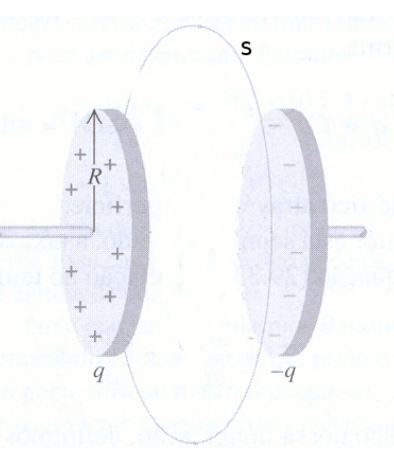
\includegraphics[scale=0.5]{figures/capacitor.png}
\end{figure}    

\begin{itemize}
\item[(A)] Zero
\item[(B)] 1,0 A
\item[(C)] 1,5 A
\item[(D)] 3,0 A
\item[(E)] 4,5 A
\end{itemize}

\vspace{0.5cm}

\textcolor{red}{\textbf{Solução:}}\\

A corrente de deslocamento de Maxwell é dada por: 

\[
i_d = \varepsilon_0 \frac{d\Phi_E}{dt}
\]

onde:
\begin{itemize}
  \item $i_d$ é a corrente de deslocamento,
  \item $\varepsilon_0$ é a permissividade elétrica do vácuo,
  \item $\Phi_E$ é o fluxo elétrico através da superfície $S$ entre as placas do capacitor.
\end{itemize}

O fluxo elétrico é definido como:

\[
\Phi_E = E \cdot A
\]

Sabemos que entre as placas de um capacitor o campo elétrico é:

\[
E = \frac{\sigma}{\varepsilon_0} = \frac{q}{\varepsilon_0 A}
\]

Logo, o fluxo elétrico será:

\[
\Phi_E = \frac{q}{\varepsilon_0}
\]

Substituindo na equação da corrente de deslocamento:

\[
i_d = \varepsilon_0 \cdot \frac{d}{dt} \left( \frac{q}{\varepsilon_0} \right) = \frac{dq}{dt}
\]

Ou seja, a corrente de deslocamento é numericamente igual à taxa de variação da carga no capacitor. Como a taxa de variação da carga é:

\[
\frac{dq}{dt} = 3{,}0 \ \mathrm{C/s}
\]

Concluímos que:

\[
\boxed{i_d = 3{,}0 \ \mathrm{A}}
\]

A resposta correta é alternativa \colorbox{green!50}{\textbf{D}}.
\end{flushleft}

\noindent\rule{\linewidth}{0.6pt}\\

\begin{flushleft}
\textbf{\textcolor{blue}{\Large Q}}\\
\noindent

\subsection{Quest\~ao }

\begin{itemize}
\item[(A)] 
\item[(B)] 
\item[(C)] 
\item[(D)] 
\item[(E)] 
\end{itemize}

\vspace{0.5cm}

\textcolor{red}{\textbf{Solução:}}\\

A resposta correta é alternativa \colorbox{green!50}{\textbf{...}}.
\end{flushleft}


\noindent\rule{\linewidth}{0.6pt}\\

\begin{flushleft}
\textbf{\textcolor{blue}{\Large Q}}\\
\noindent

\subsection{Quest\~ao }

\begin{itemize}
\item[(A)] 
\item[(B)] 
\item[(C)] 
\item[(D)] 
\item[(E)] 
\end{itemize}

\vspace{0.5cm}

\textcolor{red}{\textbf{Solução:}}\\

A resposta correta é alternativa \colorbox{green!50}{\textbf{...}}.
\end{flushleft}
